\newpage
\section{Setup and Simulation}
\subsection{Simulation using lumerical FDTD}

The following simulation and calculation is aimed to reproduce the results of \cite{heeg} and is supposed to have a more detailed look at the estimation about percentage of near field enhancement contributing to the total measured enhancement. To improve this estimation there will be a simulated graphene surface to calculate the actual enhancement along the graphene layer compared to the rough estimation of the blue dashed area in figure \ref{fig:heeg-result}.

lumerical FDTD is a commercial software to simulate systems using the FDTD method. Using this software the experimental setup of \cite{heeg} should be built inside the software to simulate the electromagnetic field within the gold nano structure. The result of this simulation will be the enhancement of the electric field $frac{\mathbf{E}(\mathbf(r))}{E_0}$ in three dimensional space. Compared to \cite{heeg} this will give a more detailed look at the spatial electromagnetic field than just a slice at $z=40nm$ and allows at a later stage to calculate the enhancement along the graphene layer.

\begin{figure}[!h]
  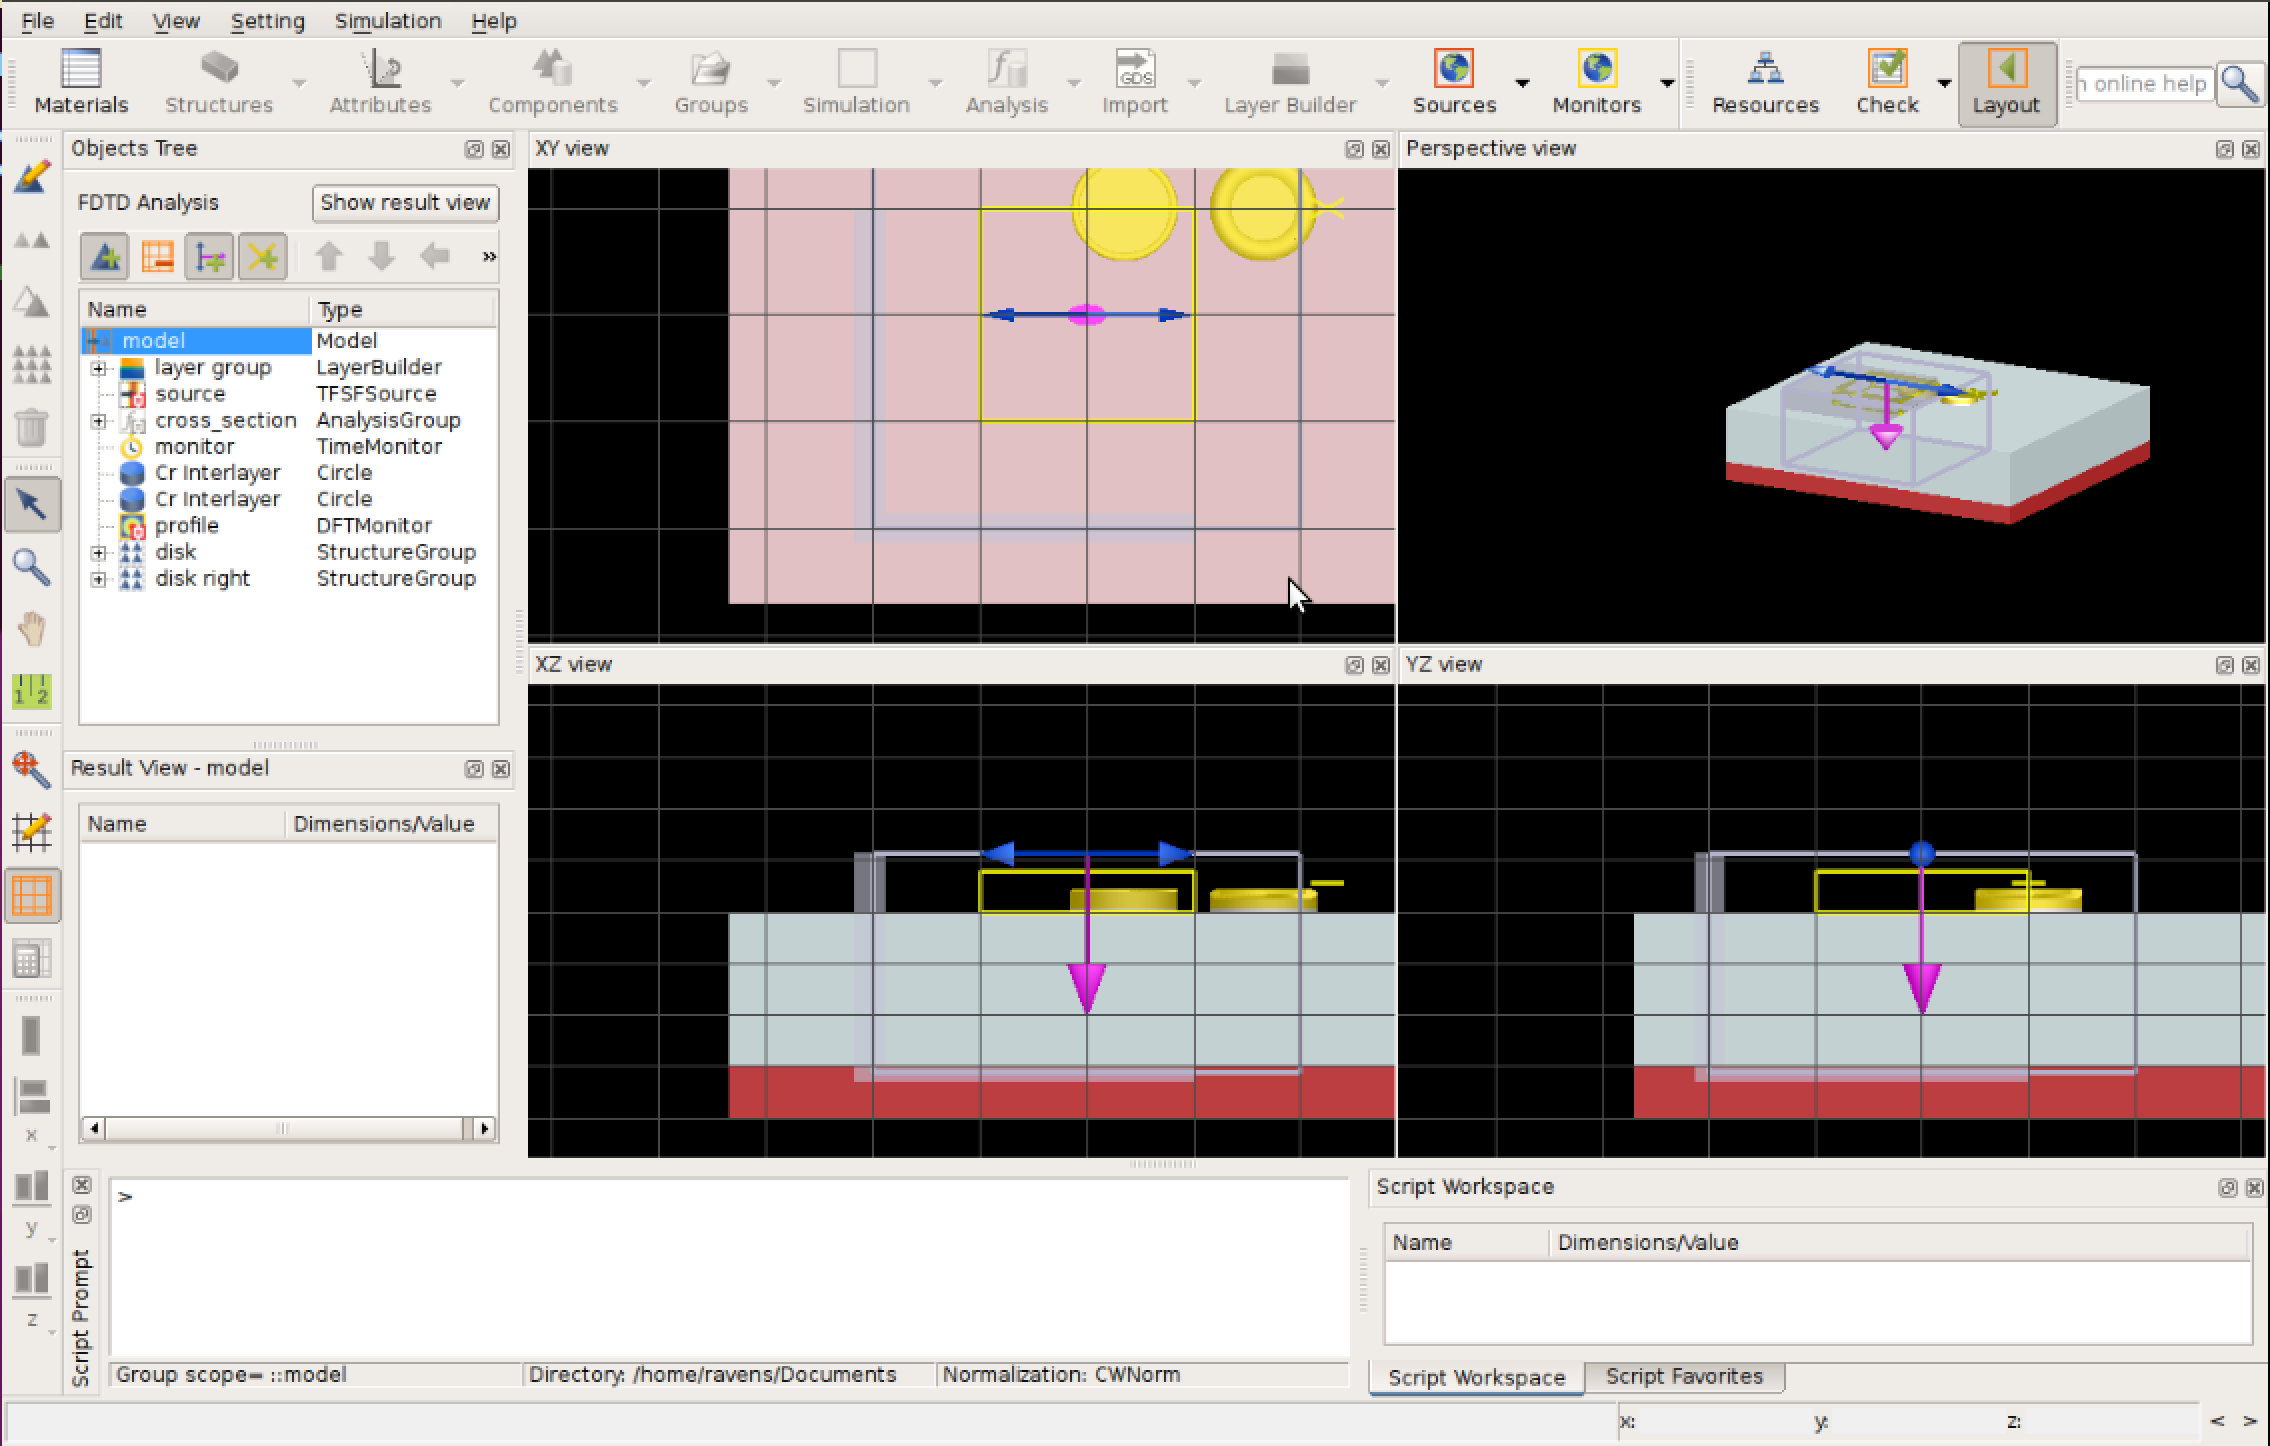
\includegraphics[width=\textwidth]{./images/lumerical.png}
  \label{fig:lumerical}
  \caption{The experimental setup of \cite{heeg} simulated in lumerical FDTD. Two gold discs with a radius of \SI{50}{nm} are placed \SI{30}{nm} apart on SiO$_2$ on a \SI{5}{nm} Cr interlayer. The upper corners of the gold discs are rounded with a radius of \SI{2}{nm}. The simulation observes an area of $\SI{400}{nm}\times\SI{400}{nm}$ with a grid size of \SI{0.5}{nm}. To improve simulation time and memory consumption, only the lower left quarter is calculated and reproduced to the other quarters by using the mirror symmetry of the system.}
\end{figure}

lumerical allows to setup different materials in 3D space using basic geometric shapes like cubes, cylinders and spheres. The base material of this experiment is a carrier layer of SiO$_2$. On this layer there are two gold nano discs of \SI{50}{nm} radius and \SI{40}{nm} height. These two discs are placed \SI{30}{nm} apart on the surface using a \SI{5}{nm} layer of Cr. The setup is done via direct entry of positions and sizes of the geometric shapes to replicate the values of Figure 1c of \cite{heeg}.

Not mentioned in \cite{heeg} is the corner radius of the gold cylinders: The real nano structure is not a perfect cylinder, therefore the simulations will be done with two different corner radiuses of \SI{2}{nm} and \SI{5}{nm}. Due to the spatial discretization there are no perfectly rounded corners anyway but rectangular aproximations. On sharp corners within the structure these aproximations become visible as small high intensity maximas.

By default the boundaries of a FDTD simulation are reflecting all magnetic and electric fields. In this experiment we observe a surface that can be approximated as infinite compared to the gold structure that is used in the measurement. To account for this the electric field leaving the simulated area is assumed to be absorbed by a Perfectly Matched Layer (PML for short).

To save time during the FDTD simulation the mirror symmetry along the $x$ and $y$ is used. This reduces the needed memory and time of the simulation by $\frac{3}{4}$, leading to a significant improvement in iteration speed. Only the left bottom quarter of the experiment is simulated (see figure \ref{fig:symmetry}).

The grid size within the simulated area is set to a uniform equidistant grid with a mesh size of \SI{0.5}{nm} between the simulated points in $x$, $y$ and $z$ direction. The total simulated area on the bottom left is a square of \SI{200}{nm}, leading to a total calculateable square of \SI{400}{nm} after mirroring the simulated results.

The simulated light pulse is a femto second pulse with a wavelength of $\lambda=\SI{638}{nm}$, matching the resonance of the plasmonic antennas \cite{heeg}.

Simulating the described system takes about 8 hours on the used machine and leads to a file size of \SI{1.24}{GB} simulated data per simulation. This simulation is done for both \SI{2}{nm} and \SI{5}{nm} corner radius. Unless otherwise noted the following sections will use data from the \SI{2}{nm} simulation.

To continue with calculations the simulated data is exported to matlab, including the three dimensional electric field (as complex values) and the three axes.

\begin{figure}[!h]
  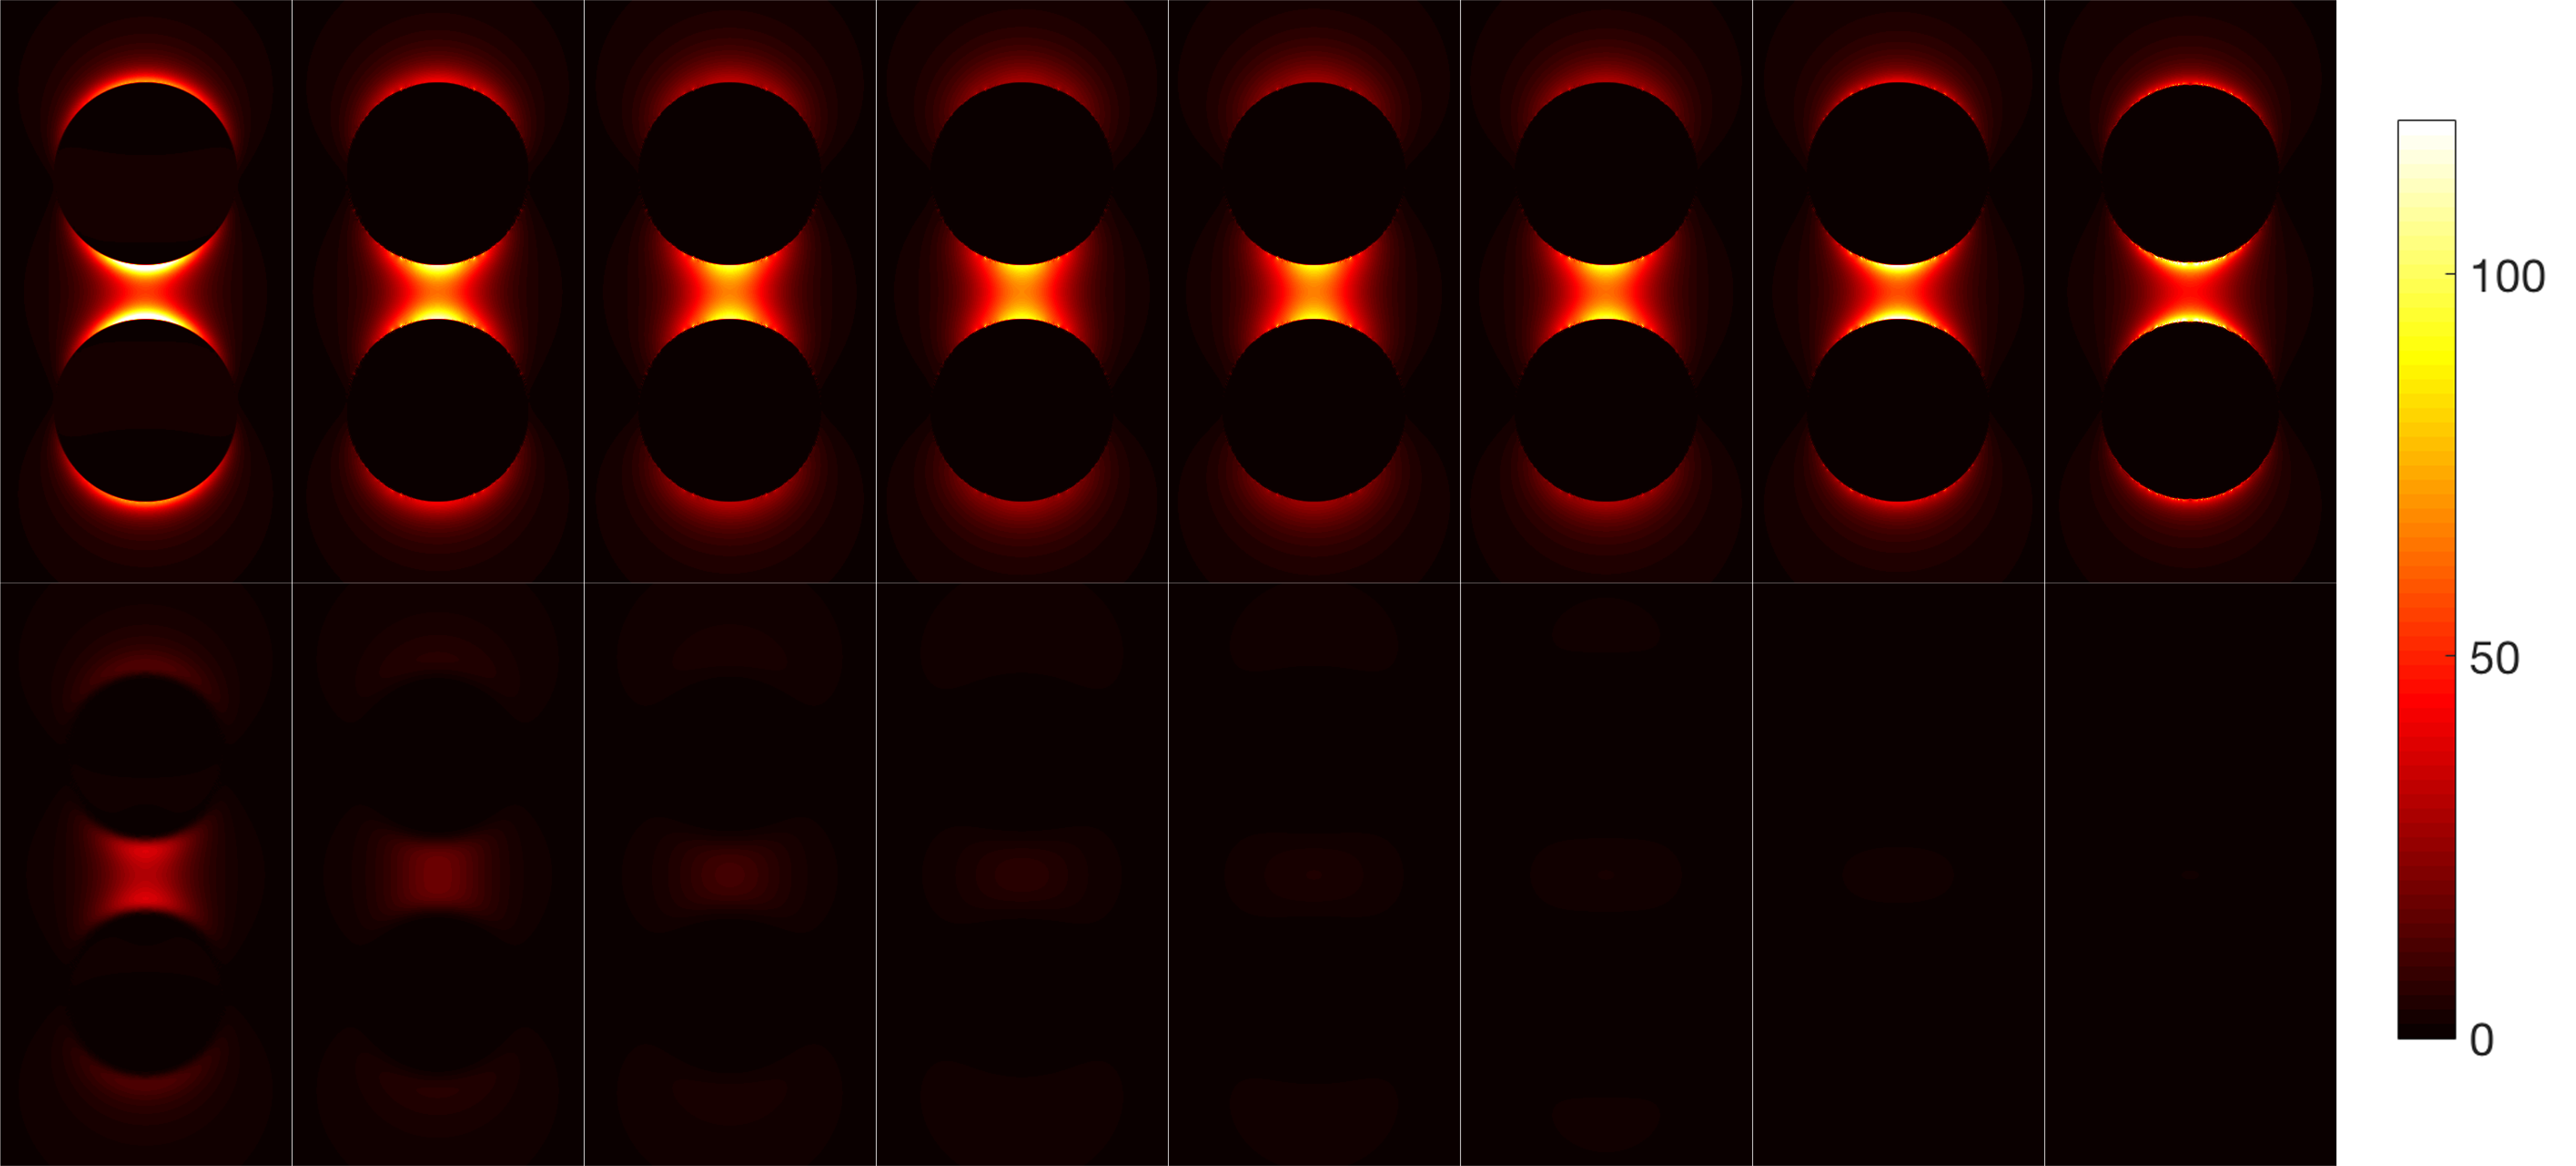
\includegraphics[width=\textwidth]{./images/simulation-slices.png}
  \label{fig:slices}
  \caption{Slices of the simulation's result in the $x,y$-plane as near field enhancement $|E/E_0|^2$. Starting at the top left at $z=\SI{0}{nm}$ continuing in \SI{5}{nm} steps until $z=\SI{80}{nm}$.}
\end{figure}
